\section{Analyse der Struktur}
In diesem Kapitel werden verschiedene dimensionierende Lastfälle vereinfacht berechnet.
Annahme bezgl. dimensionierende Lastfälle:
Diese wurde dann idealisiert und berechent um ein Gefühl für die Grössenordnung der Belastungen zu bekommen und die Grobauslegung durchführen zu können.

\subsection{Allgemeines}

\paragraph{Allgemeine Idealisierung}
SB = Vollidealisiertes Profil -> Rechteck\\
Chassis wird als zwei Längsträger idealisiert, für das Dach werden Profile angenommen. Masse des Profiles angeben inkl. Querschnittsfläche.

\subparagraph{Biegesteifigkeit}
SB ist ein Biegebalken
Widerstandsmoment nicht möglich da unterschiedlicher E-Module -> Biegesteifigkeit $EI$: Gewichtung der Biegesteifigkeiten mit E-Modul
\begin{equation}
  \label{eq:1}
  \begin{split}
    \overline{EI}_y &= \sum A_i \cdot y_i^2 \cdot E_i\\
    \overline{EI}_z &= \sum A_i \cdot z_i^2 \cdot E_i
  \end{split}
\end{equation}
Spannungen:

\begin{equation}
  \label{eq:2}
  \begin{split}
    \sigma &= \frac{M_{b,y}}{\overline{EI}_y}\cdot E_i \cdot y_i\\
    \sigma &= \frac{M_{b,z}}{\overline{EI}_z}\cdot E_i \cdot z_i
  \end{split}
\end{equation}

Schubfluss??? Wie verhält der? Idealisierung?

\paragraph{Massenverteilung}\mbox{}\\
Die vermutlich grössten Belastungen, welchen der Solar Butterfly ausgesetzt wird, entstehen aufgrund der Trägheitskräfte welche durch Beschleunigungen entstehen. Aus diesem Grund wird die Massenverteilung des Solar Butterflys genauer betrachtet. Für die festlegung der Massenverteilung wird angenommen, dass die in der Anforderungsliste definierte Maximalmasse von 3000 kg erreicht wird. Die besagte Masse wird auf insgesamt sechs Bereiche aufgeteilt; Deichsel (Bereich 0-1), Küche (1-2), Hauptkörper (2-3), Bad (3-4) und die beiden Träger A (2) und B (3).
% \begin{center}
%   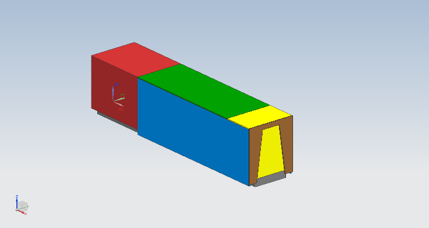
\includegraphics[width=0.5\textwidth]{04_Figures/A.png}
%   \captionof{figure}{Modus A}
%   \label{Modus A}
% \end{center}
Die Massenverteilung wurde basierend auf dem GEWICHTSEXCEL aus der Arbeit von HUBER abgeschätzt.

\subsection{1.1 Vertikale Beschleunigung}
\label{1.1 Vertikale Beschleunigung}
  \paragraph{Idealisierung}\mbox{}\\
  Um die Spannungen in der Struktur, welche aufgrund der vertikalen Beschleunigung entstehen berechnen zu können, wird der Solar Butterfly als Biegebalken mit dem in der Abbildung REF dargestelltem vollidealisiertem Querschnitt idelaisiert. \emph{A\_Dach} und \emph{A\_Chassis} stehen dabei für die Querschnittsflächen der Profile. \emph{z\_Dach} und \emph{z\_Chassis} stehen für den Abstand der Profile zum Flächenschwerpunkt. Das Profil des Chassis ist bereits vordefiniert und muss in der Grobauslegung nicht dimensioniert werden. Für die Längsträger des Daches wird für eine erste Iteration der Berechnungen ein 50x25-Rechteckprofil mit einer Wandstärke von 2 mm verwendet.\\
  Die Lagerung des Biegebalkens ist in der Abbildung REF dargestellt.

  % \begin{center}
  %   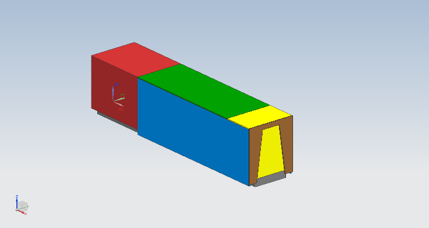
\includegraphics[width=0.5\textwidth]{04_Figures/A.png}
  %   \captionof{figure}{Modus A}
  %   \label{Modus A}
  % \end{center}

  \paragraph{Querkraft- und Biegemomentenverlauf}\mbox{}\\
  Aus der Massenverteilung und der vertikalen Beschleunigung können die Streckenlasten pro Abschnitt, die Gewichtskräfte der Träger A und B sowie die Lagerreaktionen berechnet werden. Aus ihnen können durch integration wiederum der Querkraft- und Biegemomentenverlauf berechnet werden, welche in der Abbildung REF dargestellt sind.

  \paragraph{Spannungen und Kräfte}\mbox{}\\
  Die Spannungen in den Profilen werden mit der Formel \ref{eq:2} berechnet. Bei einem maximalen Biegemoment von xxxxx kNmm ergeben sich Spannungen von xx MPa im Chassis, sowie xxx MPa im Dachträger was Kräften von xxx kN, respektive xxx kN entspricht.


  Schubfluss:
  Falls SB offen: Schubfluss muss an den Wänden der Küche und Bad abgetragen werden.

  Die Normalspannungen in den Profilen sowie die Schubspannungen in den Wänden werden als unkritisch beurteilt.

\subsection{1.2 - Longitudinale Beschleunigung negativ}
Für die Berechnung der Belastung durch longitudinale Beschleunigungen wird lediglich der Lastfall 1.2 betrachtet, da die longitudinale Beschleunigung im Lastfall 1.3 tiefer liegt als jene im Lastfall 1.2. Die Änderung des Vorzeichens der Beschleunigung im Lastfall 1.3 hat keine Auswirkung auf den Betrag der Belastung, da die Lasteinleitungen die Selbe bleibt.

  \paragraph{Idealisierung}\mbox{}\\
  Bei einer Verözerung des Solar Butterflys wird angenommen, dass die Trägheitskräfte des Aufbaus über die Seitenwände (Feld A und Feld B vgl. Abbildung [REF]) auf das Chassis abgetragen werden. Der Solar Butterfly wird als "offen" betrachtet, sodass die Seitenwände der ausfahrbaren Modulen keine Schubkärfte aufnehmen. Das Chassis  wiederum wird über Bremskräfte in der Deichsel und den Räder verzögert. Die Druckspannungen im Chassis liegen im schlimmsten Fall (Verzögerung nur duch Deichsel-Bremmskraft) tiefer als 10 MPa und werden nicht weiter untersucht.\\
  Eine weitere Annahme welche getroffen wird ist, dass die Masse über die Höhe des Solar Butterflys gleichmässig verteit ist. Weiter wird die Masse des Hauptteils und der Ausfahrmodule (Bereich 2-3) gleichmässig auf die beiden Felder A und B verteilt.

  \paragraph{Kräfte und Spannungen}\mbox{}\\
  Die Felder A und B werden wie in der Abbildung REF idealisiert. Die Kraft $F_a$ und $F_b$ ergeben sich aus der Masse des Solar Butterflys ohne Chassis und der herrschenden Beschleunigung. Die Lagerreaktionen und Schubkräfte sind in der Abbildung REF dargestellt.

\subsection{1.4 Laterale Beschleunigung}
  \paragraph{Idealisierung}\mbox{}\\
  Für den Lastfall der lateralen Beschleunigung wird der Solar Butterfly wie im Kapitel \ref{1.1 Vertikale Beschleunigung} als Biegebalken idealisiert. Da davon ausgegangen wird, dass sich der Schwerpunkt des Solar Butterflys auf einer ähnlichen Höhe wie der Flächenschwerpunk des idealisierten Querschnittes befindet, wird vereinfacht angenommen, dass die lateralen Trägheitskräfte im Flächenschwerpunk angreifen. So kommt es zu keiner Verdrehung des Biegebalkens was den Rechenaufwand reduziert. Die Lagerung des idealisierten Solar Butterflys ist in der Abbildung REF dargestellt.

  \paragraph{Querkraft- und Biegemomentenverlauf}\mbox{}\\
  Aus der Massenverteilung und der Beschleunigung können die Lagerreaktionen sowie die Trägheitskräfte berechnet werden. Der daraus resultierende Querkraft- und Biegemomentenverlauf ist in der Abbildung REF dargestellt.



  \paragraph{Träger}\mbox{}\\
  1/4 der Masse, Normalverteilt, Querkraft- und Biegemomentenverlauf
  Spannungen:

\subsection{1.5 Rotatorische Beschleunigung}












% \section{Komponenten und Verbindungen}
% In diesem Kapitel wird beschrieben, wie der Solar Butterfly aufgebaut ist. Es werden verschiedene Komponenten eingeführt und analysiert wie diese Komponenten miteinander Verbunden sind und welche Kräfte die Verbindungen übertragen müssen.\\
% Weiter wird beschrieben, wie der SB vereinfacht betrachtet wird (Biegebalken) in zwei Moden. (A und C)
%
% \subsection{Komponenten}
% bla bla
%
% \paragraph{Hauptkörper}
% Ganzer Körper als einen Kasten betrachten
% \begin{description}
%   \item \textbf{Chassis}\\
%   Idealisierung: Beam
%   \item \textbf{Boden}\\
%   Auslegung: Biegebalken
%   Idealisierung: Schalenkörper\\
%   \item \textbf{Stützen A und B}\\
%   Auslegung: Schubwand mit Türe\\
%   Profile nehmen Kräfte auf, geben diese Jedoch an die Schubwand weiter\\
%   \item \textbf{Dach}\\
%   Panelen: Schubfläche\\
%   Dach an sich: Biegebalken (Durch eigengewicht)
%   Im Modus \emph{C} Kräfte auf nehmen durch Verriegelung der Seitenwände
% \end{description}
%
% \paragraph{Seitenmodul}
% \begin{description}
%   \item \textbf{Boden}\\
%   Biegebalken und Schubfläche
%   \item \textbf{Seitenwand}\\
%   Modus A: Schubwand\\
%   Modus C: Keine
%   \item \textbf{Ausfahrmechanismus (Scharniere)}\\
%   Wand: Schubwand
%   \item \textbf{}\\
%   \item \textbf{}\\
% \end{description}
